\chapter{Experiments} \label{ch:res}
In this Chapter, first we present our models and ideas,  and dataset what we worked on. Then we present the 
related work in the contextual recommendation topic and examine their performance. Finally we 
introduce our  models and compare them with known baseline algorithms. 

\section{Datasets}
\subsection{Twitter}
Twitter is a micro bloging  service, where users can post their short messages, so called \emph{tweets} 
for the public. They are also able to follow each other profile to be get noticed after new tweets. 
Users can use \emph{\#hashtags} to inform the readers about the topics in the tweet. Further more they 
able to sign other users with \emph{\@mention}.These features makes tweeter data suitable for several 
machine learning and data mining experimenting.

The dataset, what we examined, was gathered between February 1 2012 and January 1 2013
through Twitter's streamingAPI \cite{twitterapi} by Dobos et al.\cite{dobos2013multi}
and was restricted only to geo-tagged tweets. The dataset consists of more that 1.4 billion 
tweets, including the original tweets of around 30 million retweets. After data cleansing 
and filtering a the data our final data set contains $2 993 183$ event produces by $792 860$ user
using $792 860$ hashtags.
\subsection{30M}
Turrin et al.\cite{turrin30music} introduced the 30M data set, collected through the Last.fm public API.
Their purpose was to make a public feature rich data set to the research community. 

30M  data contains: 
\begin{itemize}
    \item 31 351 954 play events
    \item 2 764 474 sessions, where a session contains series of events
    \item 47 561 User defined playlists
    \item Track features like \emph{tags}, \emph{artists} and \emph{albums}
\end{itemize}

\begin{figure} \label{fig:30m-data}
\centering 
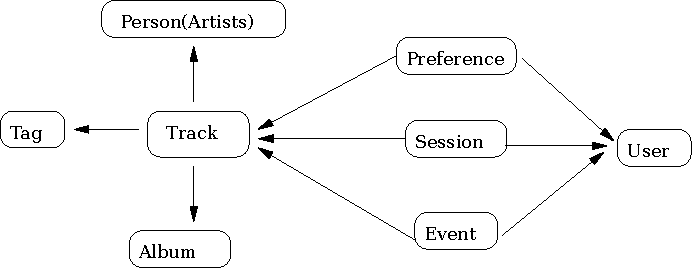
\includegraphics[scale=1]{tex/pic/30m_data_structure.pdf}
\caption{Entities and their relations in 30M}
\end{figure}


\begin{figure}[''placement specifier''] \label{fig:online}
\centering 
\includegraphics[scale=0.8]{tex/pic/time_first_hashtag.pdf}
\caption{Twitter event frequency graph on the original data and used part signed with blue}
\end{figure}
\cite{dobos2013multi}


\section{Using factor model}
\subsection{Task}
\subsection{Data}
\subsection{Batch and online experiments}

\section{Attribute based recommendation}
Each item $i$ has an attribute set $\mathcal{A}_{i}$, which contains every attribute corresponds 
to the given item. In our model a factor belongs to each attribute, this factor is independent 
from the user and the item. When we want to compute the score for a given user item $(u,i)$ pair, 
we use the already described factor model and additionally we compute the user attribute relation by 
multipile the user factor with each attribute vector belongs to the item $i$.

\subsection{Task}
\subsection{Model}
\[\hat{r}_{ui}=p_u q_i+\sum_{a\in\mathcal{A}_i}p_u f_a\]
\subsection{Experiments}

\section{Models using location}
\subsection{Task}
We can have information about users or items location. Location information have different types. Let us 
consider a restaurant, if we know where the restaurant is we will know it after a day too, but in case of
a user post a hashtag on a certain location, we only know the user \emph{current} location and nothing about 
her future positions. We can even say less about the hashtags, because a they are used by several user
and their location are different. In generally we can distinguish \emph{fix}, \emph{changing} and 
\emph{not defined} spacial items. In this Section we detailed our result \cite{palovics1location}  within we 
focused on using hashtag locations to improve the  hashtag recommendation for users. The event when a user 
$u$ post a hashtag $h$ on a location $l$ at a given time $t$ can described with 
the $(t,u,h,l)$  four. 
\subsection{Model}
In our model we assumed that we have a predefined recommender $s\left(h,n,t\right)$,
which one can predict the score of a hashtag in a given node at a given time $t$. In this case our prediction 
is the weighted sum of the predictions on the nodes from $Path(l)$, where $Path(l)$ is the set of nodes from 
location $l$ to the root node.

\[\hat{r}_{t,u,h,l}=\sum_{n\in Path\left(l\right)}w_n\cdot s\left(h,n,t\right)\]

The $w_n$ weights depend only on the nodes. We learnt the $w_n$ values by gradient descent optimizing for RMSE, 
these values 

\subsubsection{Hashtag recency}
\begin{figure}[''placement specifier''] \label{fig:online}
\centering 
\includegraphics[scale=0.8]{tex/pic/interevent.pdf}
\end{figure}
Inter even distribution for hashtag appearance is follow power-low distribution, 
$P\left(\tau=t\right)=\left(\alpha-1\right)t^{-\alpha}$, whence we can compute the probability of 
the event between $t$ and $t+\Delta t$, if the last appearance  was in $t$.

\[P\left(t<\tau\leq t + \Delta t | \tau> t\right) = 1-\left(1 + \frac{\Delta t}{t}\right)^{1-\alpha}\]

\subsubsection{Temporal popularity}
\subsection{Data}
\subsubsection{GADM tree}
We needed a detailed resulution of the earth for our location aware recommendations. We found and crawled 
 the \emph{Database of Global Administrative Areas}\cite{gadm}. This data set contains most of 
 the administrative areas in different levels for each country, for instance in US, the levels are states, counties cities, and districts. This kind of subdivision of the word implies a tree view of the world, where each node a administration area and the edges between two node means that one of the nodes is in the next  administration level and contain the other one. 
 
 After we collected and parsed the dat, we got a tree for each country. Because we wanted to connect 
 the countries to make one connected tree over the world, we added continents as nodes and a root node which represented the whole world and connected them properly \ref{fig:tree-viz}. Finally the prepared tree contained about 214 thousand  nodes and 190 thousand were leaves from them. 
 
 Our twitter data  contains only GPS coordinates for a given event and the tree did not contained coordinates, so we
 used the Google's Geocoding API \cite{geocoding} to find the coordinates for the nodes. After this we were able to order events to leaves of the GADM tree. This is how we got the \emph{GADM tree}.
 
 \begin{figure}
        \centering
\begin{tikzpicture}[sibling distance=40pt, level distance=40pt]
  \node {World}
    child {node {Europe}
      child {node {Hungary}
        child {node {Budapest}
        child {node {$\ell = {}$\ldots}}
        child {node {\ldots}}
        }
        child {node {Gy\H{o}r}
        }
        child {node {\ldots}}
      }
      child {node {Austria}
      }
      child {node {\ldots}}
    }
    child {node {Africa}}
    child {node {Asia}}
    child {node {\ldots}
    };
\end{tikzpicture}
\caption{First three levels of the tree and the user location $\ell$.}
\label{fig:tree-viz}
\end{figure}
\subsection{Experiment}

\section{Models using session informations}
\[\hat{r}_{u,i}=p_uq_i + p^{,}_uq_{i}\]







